%\documentclass[smaller,handout]{beamer}
% \documentclass[smaller,handout]{beamer}
%  \usepackage{handoutWithNotes}
% \pgfpagesuselayout{2 on 1 with notes}[letterpaper, landscape, border shrink=4mm]

\def\bmode{2} % Mode 0 for presentation, mode 1 for a handout with notes, mode 2 fo% r handout without notes
\if 0\bmode
\documentclass[smaller]{beamer}
\else \if 1\bmode
\immediate\write18{pdflatex -jobname=\jobname-Handout-Notes\space\jobname}
\documentclass[smaller,handout]{beamer}
\usepackage{handoutWithNotes}
\pgfpagesuselayout{2 on 1 with notes}[letterpaper, landscape, border shrink=4mm]
\else \if 2\bmode
\immediate\write18{pdflatex -jobname=\jobname-Handout\space\jobname}
\documentclass[smaller,handout]{beamer}
\fi
\fi
\fi

%%%%%%%%%%%%%%%%%%%%%%%%%%%%%%%%%%%%%%%%%%%%%%%%%%%%%%%%%%%%%%%%%%%%%%%%%%%%%%%%%%%%%%%%%%%%%
\newcommand{\coursetitle}{CEE 616: Probabilistic Machine Learning}
\newcommand{\longlecturetitle}{M2 Linear Methods: L2d Ridge and Lasso Regression}
\newcommand{\shortlecturetitle}{L2d: Ridge \& Lasso Regression}
\newcommand{\instructor}{Jimi Oke}
\newcommand{\lecturedate}{October 9, 2025}
%%%%%%%%%%%%%%%%%%%%%%%%%%%%%%%%%%%%%%%%%%%%%%%%%%%%%%%%%%%%%%%%%%%%%%%%%%%%%%%%%%%%%%%%%%%%%

  
\usetheme{Madrid}
\useoutertheme[subsection=false]{miniframes} % Alternatively:
                                % miniframes, infolines, split
\AtBeginSection[]{\subsection{}}

\useinnertheme{circles}
 \usepackage[backend=biber,style=authoryear,maxcitenames=2,maxbibnames=99,safeinputenc,url=false, eprint=false]{biblatex}
%\addbibresource{bib/references.bib}
% \AtEveryCitekey{\iffootnote{{\tiny}\tiny}{\tiny}}
 
 \usepackage{tipa}
% \usepackage{enumerate}
\definecolor{darkcandyapplered}{HTML}{A40000}
\definecolor{lightcandyapplered}{HTML}{e74c3c}

 

% Reduce size of frame box
\setbeamertemplate{frametitle}{%
    \nointerlineskip%
    \begin{beamercolorbox}[wd=\paperwidth,ht=2.0ex,dp=0.6ex]{frametitle}
        \hspace*{1ex}\insertframetitle%
    \end{beamercolorbox}%
}

 
% % Euler for math and numbers
% %\usepackage[euler-digits,small]{eulervm}
% %\AtBeginDocument{\renewcommand{\hbar}{\hslash}}
\usepackage{graphicx,multirow,booktabs}
\usepackage{animate}
\usepackage{media9}


% %\mode<presentation> { \setbeamercovered{transparent} }

\setbeamertemplate{navigation symbols}{}
\makeatletter
\def\beamerorig@set@color{%
  \pdfliteral{\current@color}%
  \aftergroup\reset@color
}
\def\beamerorig@reset@color{\pdfliteral{\current@color}}
\makeatother


% %=== GRAPHICS PATH ===========
\graphicspath{{./m2-images/}}
% % Marginpar width
% %Marginpar width
% %\setlength{\marginparsep}{.02in}


% %% Captions
% % \usepackage{caption}
% % \captionsetup{
% %   labelsep=quad,
% %   justification=raggedright,
% %   labelfont=sc
% % }

% \setbeamerfont{caption}{size=\footnotesize}
% \setbeamercolor{caption name}{fg=darkcandyapplered}

% %AMS-TeX packages

\usepackage{amssymb,amsmath,amsthm,mathtools} 
\usepackage{bm}
\DeclareMathOperator*{\argmax}{arg\,max}
\DeclareMathOperator*{\argmin}{arg\,min}
% \usepackage{color}

% %https://tex.stackexchange.com/a/31370/2269
\usepackage{mathtools,cancel}

\renewcommand{\CancelColor}{\color{red}} %change cancel color to red

\makeatletter
\let\my@cancelto\cancelto %copy over the original cancelto command
\newcommand<>{\cancelto}[2]{\alt#3{\my@cancelto{#1}{#2}}{\mathrlap{#2}\phantom{\my@cancelto{#1}{#2}}}}
% redefine the cancelto command, using \phantom to assure that the
% result doesn't wiggle up and down with and without the arrow
\makeatother


% %\usepackage{comment}
\usepackage{hyperref,enumerate}
% \usepackage{minitoc,array}

\definecolor{slblue}{rgb}{0,.3,.62}
% \hypersetup{
%     colorlinks,%
%     citecolor=blue,%
%     filecolor=blue,%
%     linkcolor=blue,
%     urlcolor=slblue
% }

% \usepackage{epstopdf}
% \epstopdfDeclareGraphicsRule{.gif}{png}{.png}{convert gif:#1 png:\OutputFile}
% \AppendGraphicsExtensions{.gif}

% %\usepackage{listings}

% %%% TIKZ
% \usepackage{forest}
\usepackage{tikz}
\usepackage{pgfplots}
\usepackage{pgfplotstable}
%\usepackage{pgfgantt}
\pgfplotsset{compat=newest}

\usetikzlibrary{fit,arrows,shapes,positioning,shapes.geometric}
\usetikzlibrary{decorations.markings}
\usetikzlibrary{shadows,automata}
\usetikzlibrary{patterns}
\usetikzlibrary{trees,mindmap,backgrounds}
%\usetikzlibrary{circuits.ee.IEC}
\usetikzlibrary{decorations.text}
% % For Sagnac Picture
% \usetikzlibrary{%
%     decorations.pathreplacing,%
%     decorations.pathmorphing%
% }
% \tikzset{no shadows/.style={general shadow/.style=}}
% %
% %\usepackage{paralist}

% \tikzset{
%   font=\Large\sffamily\bfseries,
%   red arrow/.style={
%     midway,red,sloped,fill, minimum height=3cm, single arrow, single arrow head extend=.5cm, single arrow head indent=.25cm,xscale=0.3,yscale=0.15,
%     allow upside down
%   },
%   black arrow/.style 2 args={-stealth, shorten >=#1, shorten <=#2},
%   black arrow/.default={1mm}{1mm},
%   tree box/.style={draw, rounded corners, inner sep=1em},
%   node box/.style={white, draw=black, text=black, rectangle, rounded corners},
% } 

\newcommand{\eps}{\epsilon}
\newcommand{\bX}{\mb X}
\newcommand{\by}{\mb y}
\newcommand{\bbe}{\bm\beta}
\newcommand{\beps}{\bm\epsilon}
\newcommand{\bY}{\mb Y}

\newcommand{\osn}{\oldstylenums}
\newcommand{\dg}{^{\circ}}
\newcommand{\lt}{\left}
\newcommand{\rt}{\right}
\newcommand{\pt}{\phantom}
\newcommand{\tf}{\therefore}
\newcommand{\?}{\stackrel{?}{=}}
\newcommand{\fr}{\frac}
\newcommand{\dfr}{\dfrac}
\newcommand{\ul}{\underline}
\newcommand{\tn}{\tabularnewline}
\newcommand{\nl}{\newline}
\newcommand\relph[1]{\mathrel{\phantom{#1}}}
\newcommand{\cm}{\checkmark}
\newcommand{\ol}{\overline}
\newcommand{\rd}{\color{red}}
\newcommand{\bl}{\color{blue}}
\newcommand{\pl}{\color{purple}}
\newcommand{\og}{\color{orange!90!black}}
\newcommand{\gr}{\color{green!40!black}}
\newcommand{\dca}{\color{darkcandyapplered}}
\newcommand{\nin}{\noindent}
\newcommand*\circled[1]{\tikz[baseline=(char.base)]{
            \node[shape=circle,draw,thick,inner sep=1pt] (char) {\small #1};}}

\newcommand{\bc}{\begin{compactenum}[\quad--]}
\newcommand{\ec}{\end{compactenum}}

\newcommand{\p}{\partial}
\newcommand{\pd}[2]{\frac{\partial{#1}}{\partial{#2}}}
\newcommand{\dpd}[2]{\dfrac{\partial{#1}}{\partial{#2}}}
\newcommand{\pdd}[2]{\frac{\partial^2{#1}}{\partial{#2}^2}}
\newcommand{\pde}[3]{\frac{\partial^2{#1}}{\partial{#2}\partial{#3}}}
\newcommand{\nmfr}[3]{\Phi\left(\frac{{#1} - {#2}}{#3}\right)}
\newcommand{\Err}{\text{Err}}
\newcommand{\err}{\text{err}}

%\DeclarePairedDelimiter\ceil{\lceil}{\rceil}
%\DeclarePairedDelimiter\floor{\lfloor}{\rfloor}

%%%% GREEK LETTER SHORTCUTS %%%%%
\newcommand{\la}{\lambda}
\renewcommand{\th}{\theta}
\newcommand{\al}{\alpha}
\newcommand{\G}{\Gamma}
\newcommand{\si}{\sigma}
\newcommand{\Si}{\Sigma}


\pgfmathdeclarefunction{poiss}{1}{%
  \pgfmathparse{(#1^x)*exp(-#1)/(x!)}%
  }

\pgfmathdeclarefunction{gauss}{2}{%
  \pgfmathparse{1/(#2*sqrt(2*pi))*exp(-((x-#1)^2)/(2*#2^2))}%
}

\pgfmathdeclarefunction{expo}{2}{%
  \pgfmathparse{#1*exp(-#1*#2)}%
}

\pgfmathdeclarefunction{expocdf}{2}{%
  \pgfmathparse{1 -exp(-#1*#2)}%
}

\newcommand{\mb}{\mathbb}
\newcommand{\mc}{\mathcal}
\newcommand{\tr}{^{\top}}
\newcommand{\pe}{\pause}
 
%%%%%%%%%%%%%%%%%%%%%%%%%%%%%%%%%%%%%%%%%%%%%%%%%%%
%%%%%%%%%%%%%%%%%%%%%%%%%%%%%%%%%%%%%%%%%%%%%%%%%%%
\title[\shortlecturetitle]{ {\normalsize \coursetitle}
  \\ \longlecturetitle}
\date[\lecturedate]{\footnotesize \lecturedate}
\author{{\bf \instructor}}
\institute[UMass Amherst]{
%\titlegraphic{\hfill
  \begin{tikzpicture}[baseline=(current bounding box.center)]
    \node[anchor=base] at (-7,0) (its) {
\includegraphics[scale=.3]{UMassEngineering_vert}} ;
  \end{tikzpicture}
  % \hfill\includegraphics[height=1.5cm]{logo}
}

%https://tex.stackexchange.com/questions/55806/mindmap-tikzpicture-in-beamer-reveal-step-by-step
  \tikzset{
    invisible/.style={opacity=0},
    visible on/.style={alt={#1{}{invisible}}},
    alt/.code args={<#1>#2#3}{%
      \alt<#1>{\pgfkeysalso{#2}}{\pgfkeysalso{#3}} % \pgfkeysalso doesn't change the path
    },
  }


% https://tex.stackexchange.com/questions/446468/labels-with-arrows-for-an-equation
% https://tex.stackexchange.com/a/402466/121799
\newcommand{\tikzmark}[3][]{
\ifmmode
\tikz[remember picture,baseline=(#2.base)] \node [inner sep=0pt,#1](#2) {$#3$};
\else
\tikz[remember picture,baseline=(#2.base)] \node [inner sep=0pt,#1](#2) {#3};
\fi
}

    
\begin{document}

\maketitle

\begin{frame}
  \frametitle{Outline}
  \tableofcontents
\end{frame}



\section{Introduction}
\begin{frame} 
  \frametitle{Model selection objectives and approaches}
  \pause

  Recall the standard linear model:
  \begin{equation}
    \label{eq:1}
    Y =  w _0 +  w _1X_1 + \cdots +  w_DX_D + \epsilon
  \end{equation}
  \pause
  In selecting a linear model for fitting a dataset, our objectives are:
  \begin{itemize}[<+->]
  \item Prediction accuracy
  \item Interpretability
  \end{itemize}
  \pause
  When tasked with finding the best set of predictors, three major methods can be applied:\pause
  \begin{itemize}[<+->]
  \item Subset selection
  \item Shrinkage (e.g.\ $\ell_{1}$ regularization, $\ell_{2}$ regularization)
  \item Dimensionality reduction: projecting the $D$-dimensional space of predictors to $M$-dimensional subspace, $M< D$
  \end{itemize}
\end{frame}

\begin{frame}
  \frametitle{Model selection criteria}
  \pause
  $n$: number of observations; $p$: number of features
  \begin{enumerate}[<+->]
  \item  Adjusted $R^2$:
  \begin{equation}
    \label{eq:30}
    R_a^2 = 1 - \fr{RSS/(N-D-1)}{TSS/(N-1)}
  \end{equation}
  \item $C_p$ statistic:
    \begin{equation}
      \label{eq:18}
     C_p =  \fr1N\lt(RSS + 2 D\hat\sigma^2\rt)
    \end{equation}
  \item AIC (Gaussian case/least squares):
    \begin{equation}
      \label{eq:17}
     \text{AIC} =  \fr{1}{N\hat\sigma^2}(RSS + 2D\hat\sigma^2)
    \end{equation}
  \item BIC (Gaussian case):
      \begin{equation}
    \label{eq:14}
    \text{BIC} = \fr{1}{N\hat\sigma^2}\lt(RSS + D\hat\sigma^2\cdot \log N\rt)
  \end{equation}
\end{enumerate}

\end{frame}




%\section{Subset selection} 


%
\begin{frame}
  \frametitle{The  overfitting problem}
  \begin{block}{Claim}
    All machine/statistical learning problems are optimization problems, \pause \textbf{e.g.}
    \begin{itemize}[<+->]
    \item Minimize loss function (e.g.\ linear regression)
    \item Maximize likelihood (e.g.\ discriminant analysis)
    \end{itemize}
  \end{block}

  \pause
  \begin{alertblock}{  The overfitting problem in regression}\pause
  \begin{itemize}[<+->]
  \item Myopically increasing the number of \textbf{predictors}/\textbf{features} (or model complexity)
    may decrease the training error of a model:
    \begin{equation*}\scriptsize
      \boxed{\text{\bf \gr Reduce training loss } \pause \to \text{ \bf \gr Lower bias }
        \to \text{ \bf \rd High variance } \to \text{ \bf \rd Poor performance} }
    \end{equation*}
    \pause

    \begin{figure}[h!]
      \centering
      \includegraphics<8->[width=.88\textwidth]{overfitting}
      %\caption{Overfitting in a classification problem}
    \end{figure}
  \end{itemize}
\end{alertblock}
\end{frame}

\begin{frame}
  \frametitle{Correcting for overfitting}
  \pause
  Overfitting can be avoided by direct estimation of test error for model selection:\pause
  \begin{itemize}[<+->]
  \item Cross-validation
  \item Bootstrapping
  \end{itemize}
  \pause
  We can also \textbf{indirectly} estimate the test error using:
  \begin{itemize}[<+->]
  \item $C_p$
  \item AIC
  \item BIC
  \end{itemize}
  Subset selection (wrapper) methods can also be applied to decide on
  relevant features.

  \medskip
  \pe

  \textbf{Regularization} can also be used to shrink or eliminate irrelevant features.
\end{frame}

\begin{frame}
  \frametitle{Mitigation of overfitting via regularization}
  \pause
  We can control for overfitting by introducing a \textbf{\rd regularization term} in the loss function to be optimized:
  \pause
  \begin{equation}
    \mc{L} = \sum_{n=1}^{N} (y_n - \hat y_n)^2 + {\rd \la \sum_{d=1}^{D} f( w _d)}
  \end{equation}
  \pause
  \begin{itemize}[<+->]
  \item The regularization term penalizes the model coefficients (shrinks them to 0)
  \item Tuning parameter $\la$ modulates the impact of the penalty
  \item As $\la \to \infty$, $ w  \to 0$
  \item The best value of $\la$ can also be learned (e.g. via cross-validation)
  \item Regularization ensures that the coefficients of irrelevant predictors are sufficiently reduced and can also be used for feature selection.
\end{itemize}
\end{frame}



\begin{frame}
  \frametitle{Further perspective on ridge regression}
  \pause

  Regularization helps us solve ill-posed problems. In this case, the OLS $RSS$ is unstable. \pause

  \begin{center}
    \includegraphics<3->[width=.7\textwidth]{3rdridge}
  \end{center}
  \pause
  With the addition of the $\ell_2$ regularization, we can reduce uncertainty about the estimate.
\end{frame}

\section{Ridge regression}
\begin{frame}
  \frametitle{Ridge regression}
    As an alternative to MLE, which seeks to maximize the likelihood $\prod_{n} p(y_{n}|\bm x_{n}, \bm w)$, we can perform a \textbf{MAP} estimation to find the posterior mode: \pe
  \begin{equation}
    \hat{\bm w}_{map} = \argmax_{\bm w}  p(\bm w|\bm y, \bm X)
  \end{equation}
\pe
\begin{itemize}
\item MAP estimation mitigates overfitting\pe
\item MAP estimation with a Gaussian prior on $\bm w$ is known as
\textbf{ridge regression}\pe
\item Yields an $\ell_2$ regularization
\end{itemize}
\end{frame}

\begin{frame}
  \frametitle{Maximum a posteriori (MAP) estimation}
  \pe
  The OLS model is given by:
  \begin{equation}
    p(\bm y|\bm X, \bm \th) = \mc{N}(\bm y | \bm X\bm w, \bm\sigma^{2}\bm I)
  \end{equation}
  \pe
  In the Bayesian view, $\bm w$ is random with some \textbf{prior} distribution (assume \textbf{Gaussian}):\pe
  \begin{equation}
    p(\bm w) = \mc{N}(\bm w| \bm 0,\tau^{2}\bm I) \pe = 
\fr{1}{\sqrt{2\pi\tau^2}}\exp\lt[-\fr12(\bm w - \bm 0)\tr
\fr{1}{\tau^2}\bm I (\bm w - \bm 0)\rt]
  \end{equation}
  \pe
  According to Bayes theorem, the posterior is proportional to:\pe
  \begin{eqnarray}
    p(\bm w|\bm y, \bm X) &\propto& p(\bm y|\bm X, \bm w) p(\bm w) \\\pe
                          &\propto& e^{\lt[-\fr12\lt(\bm w-\bm 0)\tr\fr1{\tau^{2}}\bm I(\bm w - \bm 0\rt)\rt]} \cdot
                                    e^{\lt[-\fr12\lt(\bm y-\bm X\bm w)\tr\fr1{\si^{2}}\bm I(\bm y - \bm X\bm w\rt)\rt]} \\\pe
                          &=& \exp\lt[-\fr1{2\si^{2}}(\bm y - \bm X\bm w)\tr(\bm y - \bm X\bm w) - \fr1{2\tau^{2}} ||\bm w||^{2}_{2}\rt]
  \end{eqnarray}

\end{frame}



\begin{frame}
  \frametitle{MAP estimation of linear model with Gaussian prior}
  \pe
  We can express $\hat{\bm w}_{map}$ as a minimization of the negative log-posterior: \pe 
  \begin{eqnarray}
    \hat{\bm w}_{map}  &=& \argmax_{\bm w} \log\lt( \exp\lt[-\fr1{2\si^{2}}(\bm y - \bm X\bm w)\tr(\bm y - \bm X\bm w) - \fr1{2\tau^{2}} ||\bm w||^{2}_{2}\rt] \rt) \\\pe
                       &=& \argmin_{\bm w} ~ \fr1{\si^{2}} (\bm y -\bm X\bm w)\tr (\bm y - \bm X \bm w) + \fr1{\tau^{2}}||\bm w||_{2}^{2}\\\pe
                       &=& \argmin_{\bm w} ~ (\bm y -\bm X\bm w)\tr (\bm y - \bm X \bm w) + \fr{\si^{2}}{\tau^{2}}||\bm w||_{2}^{2}\\\pe
                       &=& \argmin_{\bm w} ~ RSS(\bm w) + \la ||\bm w||_{2}^{2}\pe
  \end{eqnarray}
  \begin{itemize}
      \item $\hat{\bm w}_{map} = \hat{\bm w}^{ridge}$ if $\bm w$ has a Gaussian prior (as above)
  \item $\la =  \frac{\sigma^{2}}{\tau^{2}}$ indicates the strength of the prior on $\bm w$ %(smaller $\tau^{2} %\implies$ stronger prior  $\implies$ more regularization (shrinkage or \textbf{weight decay}))
  \item The bias $w_{0}$ is not included in $||\bm w||_{2}$  as it does not contribute to the variance: \pe
    \begin{equation}
      ||\bm w||_{2}^{2} := \sum_{d=1}^{D} w_{d}^{2}
    \end{equation}
  \end{itemize}
\end{frame}

% \begin{frame}
%   \frametitle{MAP estimation of linear model with Gaussian prior}
%   \pe
%   We can express $\hat{\bm w}_{map}$ as a minimization of the negative log-posterior: \pe 
%   \begin{eqnarray}
%     \hat{\bm w}_{map}  &=& \argmin_{\bm w} ~ \fr{1}{\si^{2}} (\bm y -\bm X\bm w)\tr (\bm y - \bm X \bm w) + \fr{1}{\tau^{2}}||\bm w||_{2}^{2}\\\pe
%                        &=& \argmin_{\bm w} ~ (\bm y -\bm X\bm w)\tr (\bm y - \bm X \bm w) + \fr{\si^{2}}{\tau^{2}}||\bm w||_{2}^{2}\\\pe
%                        &=& \argmin_{\bm w} ~ RSS(\bm w) + \la ||\bm w||_{2}^{2} \qquad \text{where } \la = \frac{\si^{2}}{\tau^{2}} \pe
%   \end{eqnarray}
%   \begin{itemize}
%       \item $\hat{\bm w}_{map} = \hat{\bm w}^{ridge}$ if $\bm w$ has a Gaussian prior (as above)
%   \item $\la =  \fr{\si^{2}}{\tau^{2}}$ indicates the strength of the prior on $\bm w$ (smaller $\tau^{2} \implies$ stronger prior  $\implies$ more regularization (shrinkage or \textbf{weight decay}))
%   \item The bias $w_{0}$ is not included in $||\bm w||_{2}$, as is standard practice in regularization, to avoid penalizing the intercept since it does not contribute to the variance: \pe
%     \begin{equation}
%       ||\bm w||_{2}^{2} := \sum_{d=1}^{D} w_d^{2}
%     \end{equation}
%   \end{itemize}
% \end{frame}

\begin{frame}
  \frametitle{Ridge estimator}\pause
  The ridge regression objective (negative log-posterior) can be written also as:
  
  \begin{equation}
    \label{eq:105}
    RSS(\bm w, \la) = (\bm y - \bm X \bm w )\tr(\bm y - \bm X \bm w ) + \la \bm w \tr \bm w 
  \end{equation}

  \pause
  Taking the derivative and equating to 0, we obtain:\pause
  \begin{equation}
    \label{eq:106}\gr
    \boxed{\hat {\bm w}^{ridge} = (\bm X^T\bm X + \la \bm I)^{-1}\bm X^T\bm y}
  \end{equation}
  \pause
  where $\bm I$ is the $D\times D$ identity matrix.\pause
  \note[item]{The term ``ridge'' comes from the diagonal shape of the regularization term $\lambda \bm I$}
  \begin{alertblock}{}
    \begin{itemize}[<+->]
    \item The matrix $\bm X^T\bm X + \la \bm I$ is \textit{\rd nonsingular}, i.e.\ it is
      \textit{\rd invertible} even when $\bm X^T\bm X$ is not full rank
    \item Recall that a matrix is \textbf{full rank} if \textit{all} its columns are \textit{\rd linearly independent}
  \item The ridge regression coefficients $\hat{\bm  w}^{ridge}$ are not scale invariant: thus we \textbf{standardize} the inputs before estimation
  \item Also, the intercept $w_0$ is not regularized (variance of a column of 1's is 0)
    \item Thus the input matrix is specified as $N \times D$ instead of $N\times (D+1)$, while $\bm w$ does not include the intercept
  \end{itemize}
  \pause
 
  
  \end{alertblock}
\end{frame}


\begin{frame}
  \frametitle{Centering and scaling (normal standardization) of inputs}
  Note that because of the penalty term $ \la  \sum_{d=1}^D  w _d^2$, ridge regression is sensitive to the scaling of the parameters (unlike in least squares). \pause
  \begin{itemize}[<+->]
  \item Thus, we \textit{\rd scale} (standardize) the inputs, i.e.\pause
    \begin{equation}
      \label{eq:a}\rd
      x'_{nd} \leftarrow \pause \fr{x_{nd}}{\hat\sigma_d}
    \end{equation}
    \pause
    where $\hat\sigma_d = \sqrt{\fr1{n-1}\sum_i(x_{nd} -\ol{x}_d)^2}$; all the predictors will have an SD of 1.
  \item We also \textbf{\bl center} the inputs for convenience:\pause
    \begin{equation}
      \label{eq:b}\bl
      x'_{nd}  \leftarrow \pause x_{nd} - \ol{x}_d
    \end{equation}
    \pause
    in which case the vector $ w $ does not include the intercept which can easily be recovered by $\hat w _0 = \fr1N\sum_iy_i$
  \item Thus, when we scale and center the inputs, we perform a \textbf{\pl normal ($z$) standardization}:\pause
    \begin{equation}
      \label{eq:c}\pl
      x'_{nd} \leftarrow \pause \fr{x_{nd} - \ol{x}_d}{\hat\sigma_d}
    \end{equation}
  \end{itemize}
\end{frame}

\begin{frame}
  \frametitle{Ridge regression with standardized inputs}\pause
  We replace the inputs with their standardized versions, take the derivative of the ridge regression objective and equate to 0:\pause
  \begin{align*}
    \begin{split}
      RSS(\la) &= \sum_{n=1}^N  \lt(y_i -  w _0 - \sum_{d=1}^D
      \fr{x_{nd} - \ol x_d}{\sigma_d} w _d\rt)^2  + \\\pe
 &\qquad \la  \sum_{d=1}^D  w _d^2 \\\pause
      RSS'(\la)_{ w _0}  &= -\sum_{n=1}^N \lt(y_i -  w _0 - \sum_{d=1}^D \fr{x_{nd} - \ol x_d}{\sigma_d} w _d\rt) = 0\\\pause
      \sum_{n=1}^N \lt(y_i -  w _0\rt) -
       \cancelto<7->{0}{\sum_{n=1}^N\sum_{d=1}^D \fr{x_{nd} - \ol x_d}{\sigma_d} w _d} &= 0\\\pause
       \sum_{n=1}^N \lt(y_i -  w _0\rt) &= 0 \quad\quad
       \pause \implies\quad \boxed{\bl \hat{ w }_0  = \ol y = \pause \fr1N\sum_{n=1}^N y_i} 
    \end{split}
  \end{align*}
  \pause
  The estimate of the intercept is thus the mean response if inputs are centered
\end{frame}



\begin{frame}
  \frametitle{Ridge regression (alternate motivation)}
  \pause
  The OLS procedures find $\hat w $ which minimizes the $RSS$:\pause
  \begin{equation}
    \label{eq:100}
    RSS = \sum_{n=1}^N \lt(y_i -  w _0 - \sum_{d=1}^D x_{nd} w _d\rt)^2
  \end{equation}\pause
  Thus:\pause
  \begin{equation}
    \label{eq:102}
    \hat w  \pause = \arg\min_{ w }\lt\{\sum_{n=1}^N  \lt(y_i -  w _0 - \sum_{d=1}^D x_{nd} w _d\rt)^2  \rt\}
  \end{equation}
  \pause
  In ridge regression, we estimate the coefficients $\hat w ^{\text{ridge}}$ to minimize the $RSS$ augmented with an {\rd $\ell_2$ penalty term}:\pause
  \begin{equation}
    \label{eq:101}
    \hat w ^R \pause = \arg\min_{ w }\lt\{\sum_{n=1}^N  \lt(y_i -  w _0 - \sum_{d=1}^D x_{nd} w _d\rt)^2  + {\rd \la  \sum_{d=1}^D  w _d^2}\rt\}
  \end{equation}
\end{frame}

\begin{frame}
  \frametitle{Ridge regression (cont.)}
  \pause
  Alternatively, we can express the ridge coefficient as an optimization problem with constraints:\pause
  \begin{align}
    \label{eq:103}
    \begin{split}
      \hat w ^R &= \arg\min_{ w }\lt\{\sum_{n=1}^N  \lt(y_i -  w _0 - \sum_{d=1}^D x_{nd} w _d\rt)^2  \rt\} \\ \pause
      &    \quad  \text{ \small subject to\ }  \sum_{d=1}^D  w _d^2 \le B
    \end{split}
  \end{align}
  \pause
  \begin{itemize}
  \item \rd The constraint is a \textbf{ball} (hypersphere) constraining the size of $ w $.
  \end{itemize}

  \pause
  \bigskip
  
  In both formulations, $\la$ and $B$ are considered tuning parameters (\textit{hyperparameters}) whose optimal values can be learned \pause (e.g. via cross-validation).
  \pause

  \bigskip
  \note[item]{Notice that neither the penalty term nor the constraint include the intercept $ w _0$.}
\end{frame}



\begin{frame}
  \frametitle{Ridge regression vs. ordinary least squares}
  \pause

  \begin{figure}[h!]
    \centering
    \includegraphics<2->[width=.7\textwidth]{olsridge}
    \caption{Ridge regression estimate compared to that of OLS}
  \end{figure}
\end{frame}



\begin{frame}[fragile]
  \frametitle{Example: Ridge regression for mpg}
  We consider the \texttt{\bl mtcars} dataset, with observations taken from the 1974 \textit{Motor Trend} US magazine, comprising fuel consumption (mpg) and 10 features of automobile design and performance. Sample size: 32. \pause

  \begin{exampleblock}{Data description}\small
\begin{verbatim}
A data frame with 32 observations on 11 (numeric) variables.

[, 1]	mpg	Miles/(US) gallon
[, 2]	cyl	Number of cylinders
[, 3]	disp	Displacement (cu.in.)
[, 4]	hp	Gross horsepower
[, 5]	drat	Rear axle ratio
[, 6]	wt	Weight (1000 lbs)
[, 7]	qsec	1/4 mile time
[, 8]	vs	Engine (0 = V-shaped, 1 = straight)
[, 9]	am	Transmission (0 = automatic, 1 = manual)
[,10]	gear	Number of forward gears
[,11]	carb	Number of carburetors
\end{verbatim}
  \end{exampleblock}
\end{frame}

\begin{frame}
  \frametitle{Example: Ridge regression for mpg (cont.)}
  \begin{figure}[h!]
    \centering
    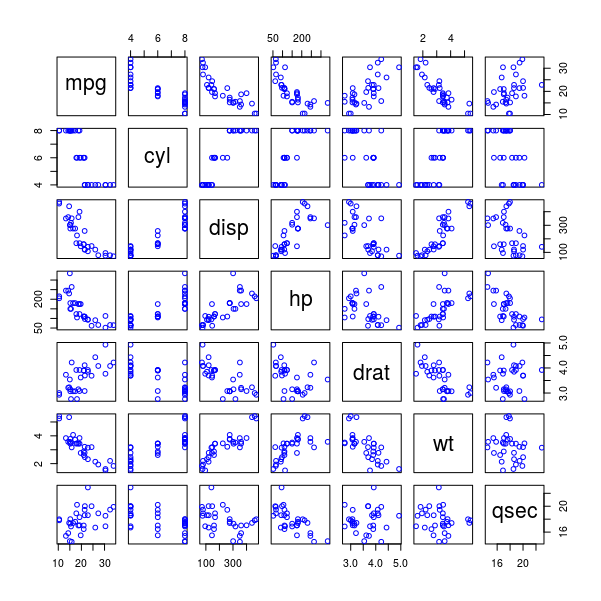
\includegraphics[width=.65\textwidth]{mtcars}
    \caption{Matrix scatterplot of selected variables in \texttt{mtcars}}
  \end{figure}
\end{frame}


\begin{frame}
  \frametitle{Example: Ridge regression for mpg (cont.)}
  \pause
  The optimal tuning parameter, $\la^*$, is learned via cross-validation (for test error estimation in each case).\pause
  
  \begin{figure}[h!]
    \centering
    \includegraphics<3->[width=.4\textwidth]{lambda-impact-1}
    \caption{Ridge regression regularization path based on MSE}
  \end{figure}

  \pause

  Here $\la^*  = 2.72$.
\end{frame}


\begin{frame}
  \frametitle{Example: Ridge regression for mpg (cont.)}
  \pause

  As $\la$ increases, the coefficients shrink to 0
    \begin{figure}[h!]
    \centering

    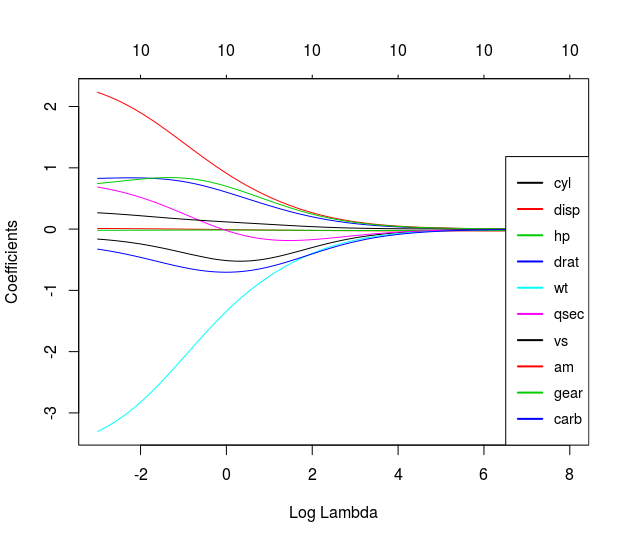
\includegraphics[width=.6\textwidth]{ridgecoef}
    \caption{Impact of $\lambda$ on ridge regression coefficient estimates}
  \end{figure}
  
\end{frame}

\begin{frame}
  \frametitle{Example: Ridge regression for mpg (cont.)}
  \pause

  The AIC and BIC can also be used to find $\la^*$:
  \pause
  \begin{figure}[h!]
    \centering

    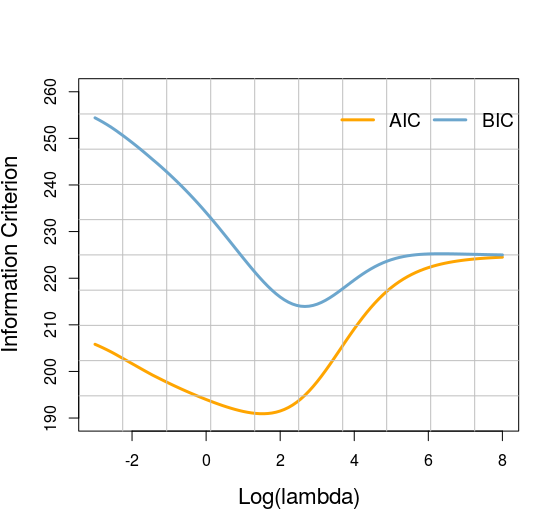
\includegraphics[width=.5\textwidth]{aicbicex2}
    \caption{Impact of $\lambda$ on ridge regression coefficient estimates}
  \end{figure}
  \pause
  Here: $\og\la^*_{\text{AIC}} = 4.7$,\qquad \pause $\bl\la^*_{\text{BIC}} = 14.4$ 
  
\end{frame}


\section{The lasso}

\begin{frame}
  \frametitle{Lasso regression}
  In lasso (\textbf{l}east \textbf{a}bsolute \textbf{s}hrinkage
  \textbf{s}election \textbf{p}rior) regression, we assume a \textbf{Laplace} prior on the parameters:\pe
  \begin{equation}
    p(\bm w|\la) = \text{Lap}(\bm w|\bm 0,  b) =\pe
\fr{1}{2b}\exp\lt(-\fr{|\bm w - \bm 0|}{b}\rt)
  \end{equation}
\pe
\begin{itemize}
\item Following the MAP estimation steps, this results in the
  following estimator: \pe
  \begin{equation}
    \hat{\bm w}_{map}^{\text{lasso}} = \argmin{\bm w} RSS(\bm w) + \la ||\bm w||_1
  \end{equation}
\pe
\item $||\bm w||_1 = \sum_{d=1}^D |w_d|$ is the $\ell_1$ norm of $\bm
  w$
\item MAP estimation with a Laplace prior is known as $\ell_1$-regularization
\end{itemize}
\end{frame}
\begin{frame}
  \frametitle{Lasso as feature selector}
  In Lagrangian form, the \textbf{\rd lasso} estimate is given by:
  \pause
  \begin{equation}
    \label{eq:107}
    \hat w ^{\text{lasso}} \pause = \arg\min_{ w }\lt\{\sum_{n=1}^N  \lt(y_i -  w _0 - \sum_{d=1}^D x_{nd} w _d\rt)^2  + {\rd \la  \sum_{d=1}^D | w _d|}\rt\}
  \end{equation}
  \pause

  % \begin{alertblock}{}
    \begin{itemize}[<+->]
    \item The lasso differs from ridge regression in that it uses $\ell_1$ instead of $\ell_2$ regularization \pause
      (\textit{\rd sparsity constraint} \pause $\to$ \textit{\rd greater interpretability})
      
      \pause
      \begin{center}
      \includegraphics<6->[width=.6\textwidth]{l1l2}
    \end{center}
    \item Thus, it forces irrelevant coefficients to zero instead of
      shrinking them
    \item And therefore acts as a \textbf{feature selector}
%  Lasso is also referred to as \textit{basis pursuit} in signal processing. \pause
    \end{itemize}
  % \end{alertblock}
\end{frame}


% \begin{frame}
%   \frametitle{Further perspective on lasso regression}
%   \pause
%   A three-dimensional illustration: \pause
  
%   \begin{center}
%     \includegraphics<3->[width=.7\textwidth]{2ndridge}
%   \end{center}
% \end{frame}

\begin{frame}
  \frametitle{Solving the lasso}
  \pause

  \begin{figure}[h!]
    \centering
    \includegraphics<2->[width=.5\textwidth]{6-7}
    \caption{Comparing the lasso and ridge regression approaches}
  \end{figure}
  \pause
  \begin{itemize}[<+->]
  \item $\hat {\bm w}^{\text{lasso}}$ has no closed form (unlike ridge regression)
  \item The optimization problem can be solved via quadratic programming (convex optimization)
  \item An algorithm (Efron et al.) for computing the lasso path: \textbf{least angle regression (LARS)}
  \item The lasso can be implemented in R using the \texttt{\rd lars} package or in Python using \texttt{LassoCV}, \texttt{LassoLarsCV} or \texttt{LassoLarsIC} modules in \texttt{sklearn}.
    
  \end{itemize}
\end{frame}



% \begin{frame}[fragile]
%   \frametitle{Correcting for collinearity (cont.)}
%   \begin{exampleblock}{Example: Regressing \texttt{Balance} on \texttt{Income}, \texttt{Limit}, \texttt{Rating} and \texttt{Age} (\texttt{Credit} dataset); cont. }\pause
%     Finally, we remove \texttt{\bl Age} ($X_4$), as it has a high p-value and hence an unreliable predictor
%     \begin{equation*}
%       Y =  w _0 +  w _1X_1 +  w _3X_3
%     \end{equation*}
%     \pause
%     The adjusted $R^2$ in this final case remains 0.875.     
%   \end{exampleblock}
% \end{frame}


\section{Subset selection}

\begin{frame}
  \frametitle{Best subset selection}
  Given a dataset with $D$ possible predictors, how many possible subsets can be selected in a linear model? \pause

  \begin{alertblock}{Number of possible linear models for a given dataset}
    In deciding on the subset, we have 2 possibilities for each predictor: include/exclude.\pause

    Since there are $D$ predictors, the total number of possibilities is:\pause
    \begin{equation}
      \label{eq:2}
      \prod_{d=1}^D 2 = 2^D
    \end{equation}    
  \end{alertblock}

  \pause

  Thus, to select the best subset of predictors, we could examine all $2^D$ possibilities (exhaustive enumeration), but this could be computationally expensive.
  \pause

  \bigskip

  Can we reduce the problem from $2^D$ possibilities to $D+1$?
\end{frame}


\begin{frame}
  \frametitle{Best subset selection algorithm}
  \begin{enumerate}[<+->]
  \item Let $\mathcal{M}_0$ be the null model containing no predictors.
  \item For $k=1,2,\ldots,D$:\pause
    \begin{enumerate}[(a)]
    \item Fit all ${D \choose k}$ models containing exactly $k$ predictors \pause
    \item Pick the model with the smallest $RSS$. Let this be $\mathcal{M}_k$ \pause
    \end{enumerate}
  \item Select a single best model from $\mathcal{M}_0, \ldots, \mathcal{M}_D$ using the CV prediction error (AIC), BIC or $R_a^2$
  \end{enumerate}
  % \begin{algorithm}
  %   \Kw
  % \end{algorithm}
\end{frame}

\begin{frame}
  \frametitle{Notes on best subset selection}
  \begin{itemize}[<+->]
  \item Can quickly get intractable if $D > 40$
  \item Can be generalized for other types of regression (e.g.\ logistic regression) and models
  \item Ultimately, $2^D$ models still have to be estimated, but only ${D \choose k}$ need to be evaluated in each step
  \end{itemize}
  \pause
  \begin{exampleblock}{Alternatives}
    \begin{enumerate}[<+->]
    \item Forward stepwise selection
    \item Backward stepwise selection      
    \end{enumerate}
  \end{exampleblock}
\end{frame}

\begin{frame}
  \frametitle{Forward stepwise selection}\pause
  As earlier discussed, this reduces the size of the best subset selection problem by evaluating a maximum of $D-k$ models in each step,
  with variables incrementally added to improve the goodness-of-fit measure in each iteration:\pause

  \begin{enumerate}[<+->]
  \item Let $\mathcal{M}_0$ denote the null model
  \item For $k = 0, \ldots, D -1$:\pause
    \begin{enumerate}[(a)]
    \item Evaluate all $D-k$ models that augment the predictors in $\mathcal{M}_k$ by 1 additional predictor
    \item Choose the best of these models (based on $R^2$, $RSS$, etc), and call it $\mathcal{M}_{k+1}$
    \end{enumerate}
  \item Select a single best model from among $\mathcal{M}_0, \ldots, \mathcal{M}_D$ using the CV prediction error (AIC), BIC or  $R_a^2$
  \end{enumerate}
  \pause
  \begin{alertblock}{Notes}
    \begin{itemize}[<+->]
    \item Forward stepwise selection can fail to find the best subset if it does not contain the predictor chosen in $\mathcal{M}_{k+1}$
    \end{itemize}
  \end{alertblock}
\end{frame}

\begin{frame}
  \frametitle{Backward stepwise selection}
  \pause
  In this case, we begin with the full model containing all $p$ predictors and then iteratively remove the least relevant predictor at each step:\pause
  
  \begin{enumerate}[<+->]
  \item Let $\mathcal{M}_D$ denote the full model containing all $p$ predictors
  \item For $k = D, D -1, \dots, 1$:
    \begin{enumerate}[(a)]
    \item Consider all $k$ models that contain all but one of the predictors in $\mathcal{M}_k$
    \item Choose the best (based on $R^2$, $RSS$, etc) among these $k$ models. Let it be $\mathcal{M}_{k-1}$
    \end{enumerate}
  \item Select a single best model from among $\mathcal{M}_0, \ldots, \mathcal{M}_D$ using the CV prediction error (AIC), BIC or  $R_a^2$
  \end{enumerate}
\end{frame}

\begin{frame}
  \frametitle{Comparing forward and backward stepwise selection}
  \pause
  \begin{itemize}[<+->]
  \item Both require the estimation of the same number of models:\pause
    \begin{equation}
      \label{eq:3}
      1+ \sum_{k=0}^{D-1}(D-k) = 1+ \fr{D(D+1)}{2}
    \end{equation}
  \item Backward selection requires $N>D$ but forward selection does not have this restriction. Why?
  \item Thus, when $D$ is large, forward selection is the viable approach
  \item Hybrid approaches combining both forward and backward steps can be implemented for flexibility and computational feasibility
  \end{itemize}
\end{frame}


\begin{frame}
  \frametitle{Example: Predicting monthly  temperature}
  \pause
  In this example, we consider monthly average temperature for Boston, MA (1978 to 2019). \pause

  \begin{figure}[h!]
    \centering

    \includegraphics<3->[width=.7\textwidth]{avetemp}
    \caption{Monthly average temperature in Boston from 1978 to 2019}
  \end{figure}
\end{frame}

\begin{frame}
  \frametitle{Example: Predicting monthly temperature (cont.)}
  \pause
  In time series regression, we might want to include the effects historical observations on the current response using \textbf{lag variables}:\pause

  \begin{align*}
    X_t & \quad \text{(observation in period t)} \\
    X_{\text{lag}_1} &= X_{t-1} \\
    X_{\text{lag}_2} &= X_{t-2} \\
    \vdots &\quad \vdots\\
    X_{\text{lag}_p} &= X_{t-p}
  \end{align*}
  where $k$ is the number of historical time periods. 
\end{frame}

\begin{frame}
  \frametitle{Example: Predicting monthly temperature (cont.)}
  \pause
  We create 12 lag variables: \texttt{T\_AVG\_LAG\_k}, \texttt{k} $=1,\ldots,12$.\pause
  \begin{figure}[h!]
    \centering
    \includegraphics<3->[width=.8\textwidth]{lagscatter}
  \end{figure}
  \pause
  Which lag variables are strongly correlated with monthly temperature?
\end{frame}

\begin{frame}[fragile]
  \frametitle{Example 1: Predicting monthly temperature (cont.)}
  \pause
  In the Jupyter notebook, we illustrate an exhaustive enumeration to select the best linear regression model using AIC:

  {\tiny\bl
\begin{verbatim}
Best expr=TAVG ~ TAVG_LAG_1 + TAVG_LAG_2 + TAVG_LAG_5 + TAVG_LAG_6 + TAVG_LAG_10 + TAVG_LAG_11 + TAVG_LAG_12
min AIC=1989.7279346561804
                            OLS Regression Results                            
==============================================================================
Dep. Variable:                   TAVG   R-squared:                       0.964
Model:                            OLS   Adj. R-squared:                  0.963
Method:                 Least Squares   F-statistic:                     1458.
Date:                Fri, 21 Feb 2020   Prob (F-statistic):          1.15e-272
Time:                        02:51:46   Log-Likelihood:                -986.86
No. Observations:                 393   AIC:                             1990.
Df Residuals:                     385   BIC:                             2022.
Df Model:                           7                                         
Covariance Type:            nonrobust                                         
===============================================================================
                  coef    std err          t      P>|t|      [0.025      0.975]
-------------------------------------------------------------------------------
Intercept      31.2917      6.126      5.108      0.000      19.247      43.337
TAVG_LAG_1      0.2809      0.047      5.915      0.000       0.188       0.374
TAVG_LAG_2      0.1038      0.042      2.461      0.014       0.021       0.187
TAVG_LAG_5     -0.1530      0.048     -3.156      0.002      -0.248      -0.058
TAVG_LAG_6     -0.2334      0.049     -4.730      0.000      -0.330      -0.136
TAVG_LAG_10     0.0780      0.044      1.786      0.075      -0.008       0.164
TAVG_LAG_11     0.1663      0.051      3.263      0.001       0.066       0.267
TAVG_LAG_12     0.1517      0.050      3.047      0.002       0.054       0.250
==============================================================================
Omnibus:                       14.731   Durbin-Watson:                   2.014
Prob(Omnibus):                  0.001   Jarque-Bera (JB):               25.147
Skew:                          -0.232   Prob(JB):                     3.46e-06
Kurtosis:                       4.149   Cond. No.                     5.53e+03
==============================================================================
\end{verbatim}
    }
\end{frame}


\begin{frame}
  \frametitle{Example: Predicting monthly temperature (cont.)}
  \pause
  We compare the fitted values to the observations in the test set using this ``best'' model.\pause
  \begin{figure}[h!]
    \centering
    \includegraphics<3->[width=.6\textwidth]{predtemp}
    \caption{Performance of ``best'' model}
  \end{figure}
  \pause
  Examine the code in the Jupyter notebook. Identify at least \textbf{3 weaknesses} of the approach used and how you would address them.
\end{frame}
 

\section{Outlook}
\begin{frame}
  \frametitle{Summary}\pause
  \begin{block}{Model performance}
    \pause
    We consider model fitness by:
    \begin{itemize}
    \item Inference (statistical tests on parameter significance)
    \item Error estimation (MSE, $R^{2}$, AIC, BIC, etc)
    \end{itemize}
  \end{block}
  
  \begin{block}{Subset selection}\pause
    Algorithms for selecting best number of features\pause
    \begin{itemize}
    \item Forward stepwise
    \item Backward stepwise
    \end{itemize}
  \end{block}
  
  \begin{block}{Regularization}\pause
    Another approach to mitigating overfitting\pause
  \begin{itemize}[<+->]
  \item Ridge regression is closed form and shrinks the coefficients to zero
  \item The lasso produces a sparse solution (effective for feature selection) as it employs $\ell_1$ regularization
  \end{itemize}
\end{block}

\end{frame}


\begin{frame}
  \frametitle{Reading assignments}

  \begin{itemize}
  \item \textbf{PMLI} 11.3-4
  \item \textbf{ESL} 3.3-7 %; ISLR 6
  \end{itemize}

  

\end{frame}


\appendix
\section{A1: LS estimators}

\begin{frame}
  \frametitle{OLS model}
  \pause
  The ordinary least squares (OLS) model is given by\pause
  \begin{equation}
    \bm Y = \bm X \bm  w  + \bm\epsilon
  \end{equation}
  \pause
  where the errors are independent and identically distributed (iid) as follows:
  \begin{itemize}
  \item $\mb{E}(\bm\eps) = \bm 0$ (zero mean)\pause
  \item $Cov(\bm\eps) = \sigma^{2}\bm I$ (constant variance)
  \end{itemize}
  \pause
  Also:\pause
  \begin{itemize}
  \item $\bm y$ and $\bm \eps$ are normally distributed random variables (r.v.'s)
    \pause
  \item $\mb{E}(\bm y) = \bm X\bm w  + \mb{E}(\bm \eps) = \bm X\bm  w $
  \end{itemize}
  \pause
  Recall the OLS estimator:
  \begin{equation}
    \hat{\bm w }_{OLS} = (\bm X^{T}\bm X)^{-1}\bm X^{T}\bm y
  \end{equation}
  \pause
  which is an \textbf{unbiased} estimator of $ w $, since \pause
  \begin{equation}
    \mb{E}(\hat{\bm w }_{OLS}) = \pause
    (\bm X^{T}\bm X)^{-1}\bm X^{T} \mb{E}(\bm y) \pause = (\bm X^{T}\bm X)^{-1}\bm X^{T}\bm X\bm w  = \pause \bm w 
  \end{equation}
\end{frame}

\begin{frame}
  \frametitle{Generalized least squares (GLS) model}\pause
  The GLS model is given by \pause
  \begin{equation}
    \bm Y = \bm X \bm  w  + \bm\epsilon
  \end{equation}
  \pause
  where \pause
  \begin{itemize}
  \item $\mb{E}(\bm\eps) = \bm 0$ (zero mean)\pause
  \item $Cov(\bm\eps) = \sigma^{2}\bm \Omega$\pause
  \item $\bm \Omega$ is a known $n\times n$ positive definite (PD) matrix (i.e. not
    necessarily constant variance)
  \end{itemize}
  \pause
  
  The GLS estimator is then given by: \pause
  \begin{equation}
    \hat{\bm w }_{GLS} = (\bm X^{T}\bm \Omega^{-1} \bm X)^{-1}\bm X^{T}\bm \Omega^{-1}\bm y 
  \end{equation}
  \pause

  Fitted values are given as \pause
  \begin{equation}
    \hat{\bm y}_{GLS} = \bm X \hat{\bm w }_{GLS}
  \end{equation}
\end{frame}
 
 
\begin{frame}
  \frametitle{Weighted least squares (WLS)}
  \pause
  Special case of GLS where\ $\bm \Omega$ is diagonal: \pause 
  \begin{equation}
    \bm \Omega = \bm W^{-1} = 
    \begin{bmatrix}
      w_{1} & \cdots & 0 \\
      \vdots & \ddots & \vdots \\
      0 & \cdots & w_{n}
    \end{bmatrix}^{-1}
    =
        \begin{bmatrix}
      \fr 1{w_{1}} & \cdots & 0 \\
      \vdots & \ddots & \vdots \\
      0 & \cdots & \fr1{w_{n}}
    \end{bmatrix}
  \end{equation} 
  where $w_{1},\ldots,w_{n}$ are weights.
  \pause

  \bigskip
  Thus, the WLS model is specified as: \pause
  \begin{equation}
    \bm y = \bm X \bm  w  + \bm\epsilon   
  \end{equation}
  where $\mb{E}(\bm\eps) = \bm 0$ and $Cov(\bm\eps) = \sigma^{2}\text{diag}\lt(w_{1},\dots, w_{n}\rt)$
  \pause
  
  And the estimator is:\pause
  \begin{equation}
        \hat{\bm w }_{WLS} = (\bm X^{T}\bm W \bm X)^{-1}\bm X^{T} \bm W \bm y
  \end{equation}
\end{frame}

\begin{frame}
  \frametitle{WLS in practice}
  \pause
  So, how do we estimate the weights to find the WLS estimator?
  \pause
  \begin{itemize}
  \item It has been shown that  $\hat{\bm w }_{WLS}$ is BLUE when: \pause
    \begin{equation}
      w_{i} = \fr{1}{\sigma_{i}^{2}}
    \end{equation}
  \item In many cases, the $i$-th squared residual $e_{i}$ is a good estimate of $\sigma_{i}^{2}$
  \item If the relationship between the residuals and fitted values indicates a megaphone shape, regress $|e_{i}|$ against the fitted values to find $\hat\sigma_{i}$
  \item If the squared residuals indicate an upward trend w.r.t predictors or fitted values, regress against to find $\hat\sigma_{i}$
  \end{itemize}
\end{frame}

\begin{frame}
  \frametitle{Feasible generalized least squares (FGLS)}
  When a diagonal covariance matrix cannot be assumed, the FGLS provides a more general approach.

  \pause

  \bigskip
  In FGLS, we assume that $\bm \Omega = \bm\Omega(\bm\theta)$, i.e.\ it is a function of an unknown vector of parameters $\bm\theta$.

  \pause

  \bigskip

  The estimator is given by: \pause
    \begin{equation}
        \hat{\bm w }_{FGLS} = (\bm X^{T}\hat{\bm \Omega}^{-1} \bm X)^{-1}\bm X^{T} \hat{\bm\Omega}^{-1} \bm y
  \end{equation}
\end{frame}
 
\end{document}

%%% Local Variables:
%%% mode: latex
%%% TeX-master: t
%%% End:
